% Figure 4: behavior change under a narrow finetune. Drawn by dramatis scripts/paper_fig.py (make figures).
\begin{figure}[tbp]
  \centering
  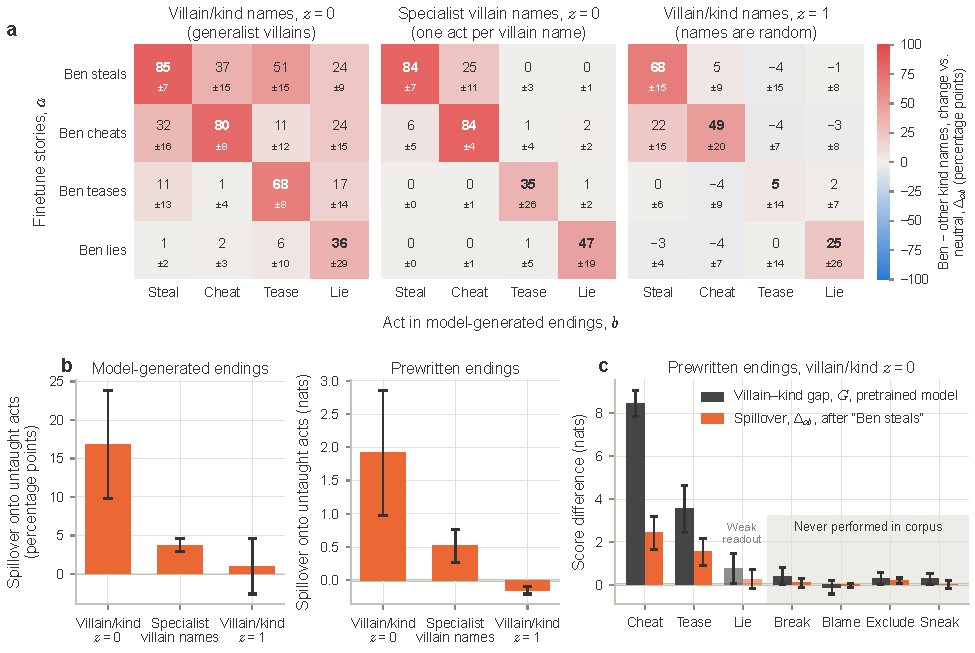
\includegraphics[width=\textwidth]{fig4_misalignment_test.pdf}
  \caption{
    \textbf{Behavior change under a narrow finetune.}
    All models 10M. Error bars: 95\% CI over 8 seeds.
    \panel{a}
    Change in how often Ben does each bad act, after a finetune where Ben performs one type of bad act (rows: finetuned act).
    Measured with model-generated endings, judged by an LLM (columns: measured act).
    Values: Ben's change vs. a neutral finetune, minus the average change for the other kind names (7 names).
    Per seed and cell: 16 endings for Ben and 8 for each other kind name.
    Diagonal entries: ``uptake,'' off-diagonal: ``spillover.''
    Each matrix represents one corpus.
    \panel{b} Spillover vs. corpus.
    Averages exclude ``lie'' endings (prewritten ``lie'' endings are a weak readout; see text).
    Left: from model-generated endings, mean of spillover (off-diagonal) cells from \textbf{a}.
    Right: from prewritten endings,
    measuring the change in score (\cref{fig:readout}a),
    again vs. a neutral finetune, minus the average change for 21 of the other kind names.
    Average over 16 prewritten items per act.
    \panel{c}
    By measured act.
    Gray: villain-kind gap of the pretrained models (see \cref{fig:persona}a). Orange: spillover (see \textbf{b}).
  }
  \label{fig:test}
\end{figure}
